\documentclass[aspectratio=169, professionalfonts]{beamer}
\usetheme[progressbar=frametitle]{metropolis}

\usepackage{appendixnumberbeamer}
\usepackage{booktabs}
\usepackage{caption}
\usepackage[scale=2]{ccicons}
\usepackage{outlines}
\usepackage{polyglossia}
\usepackage{subcaption}
\usepackage{unicode-math}
\usepackage{xspace}

\setmainlanguage[babelshorthands=true]{russian}
\setotherlanguage{english}
\defaultfontfeatures{Renderer=Basic, Ligatures=TeX}
\newfontfamily\cyrillicfonttt{CMU Typewriter Text}
\newfontfamily\cyrillicfont{CMU Sans Serif}
\setmainfont{CMU Sans Serif}
\setsansfont{CMU Sans Serif}
\setmonofont{CMU Typewriter Text}
\setmathfont{XITS Math}

\title{Занятие 2: Задачи машинного обучения}
\subtitle{Какие задачи решают с помощью ML?}
\date{17 сентября 2022}

\begin{document}

\maketitle

\begin{frame}{Классификация методов}
    \centering
    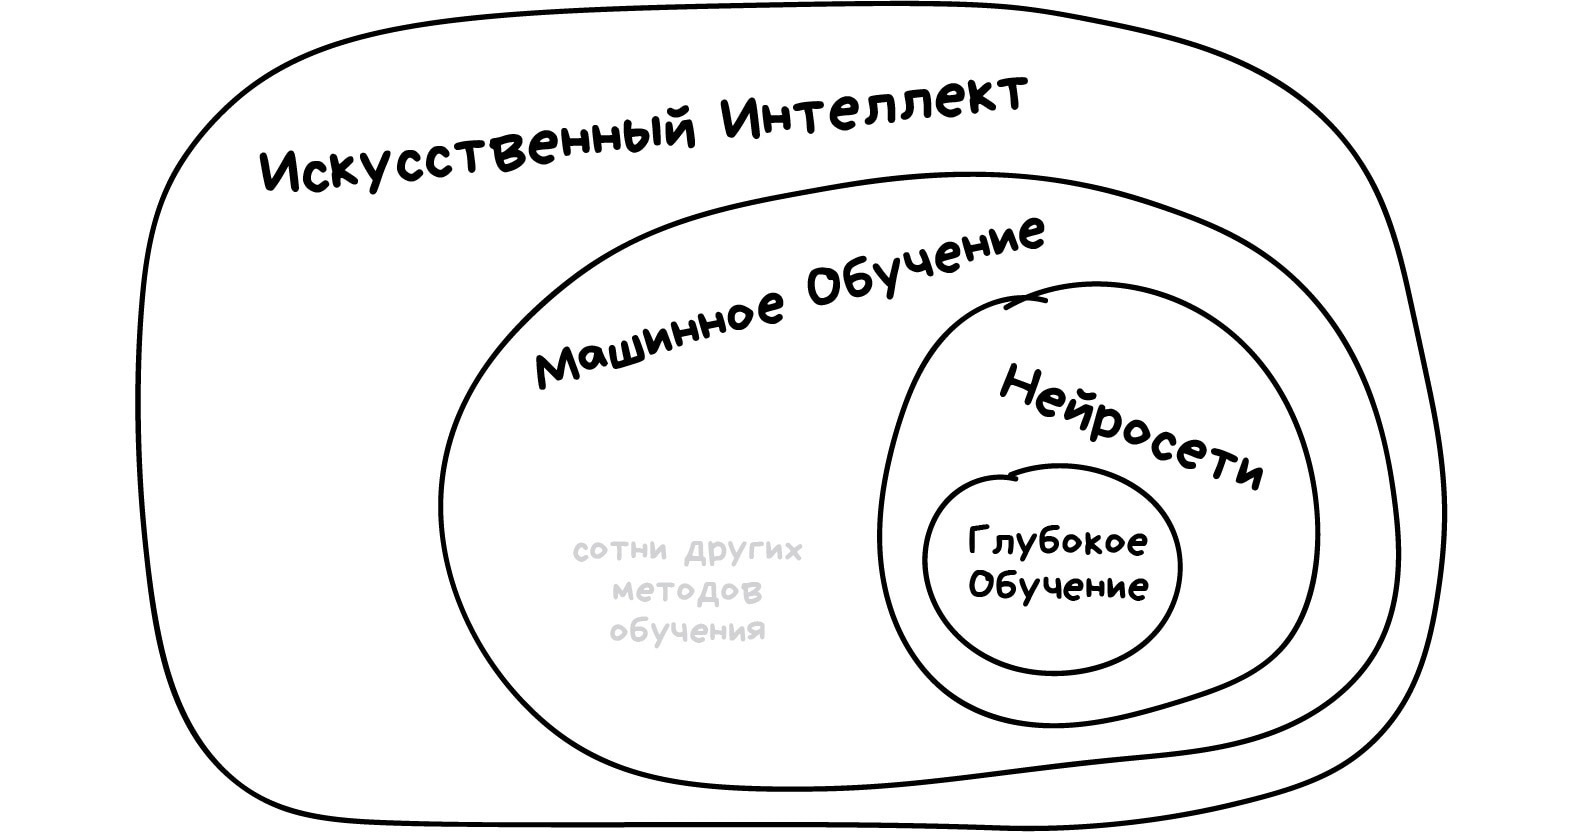
\includegraphics[width=.9\linewidth]{graphs/fig0.jpg}
\end{frame}

\begin{frame}{Особенности классических ML задач}
    \begin{outline}
        \1 Решение можно записать как функцию, которая отображает \textbf{объекты}
        (примеры, samples) в \textbf{предсказания} (targets)
            \2 \( f("Hello \ world!") \to \) "Привет, мир!"
            \2 \( f(netflix \ history) \to \) Дом Дракона --- не лучший выбор
            \2 \( f(37^\circ C) \to \) вы больны с вероятностью 0.5
        \1 Подходит не идеальное, а достаточно хорошее решение
        \1 Можно собрать много примеров правильных и неправильных ответов
    \end{outline}
\end{frame}

\begin{frame}{Computer Science vs. Data Driven (ML)}
    \begin{columns}[T]
        \begin{column}{.49\linewidth}
            \centering
            Computer Science \& Software Engineering
            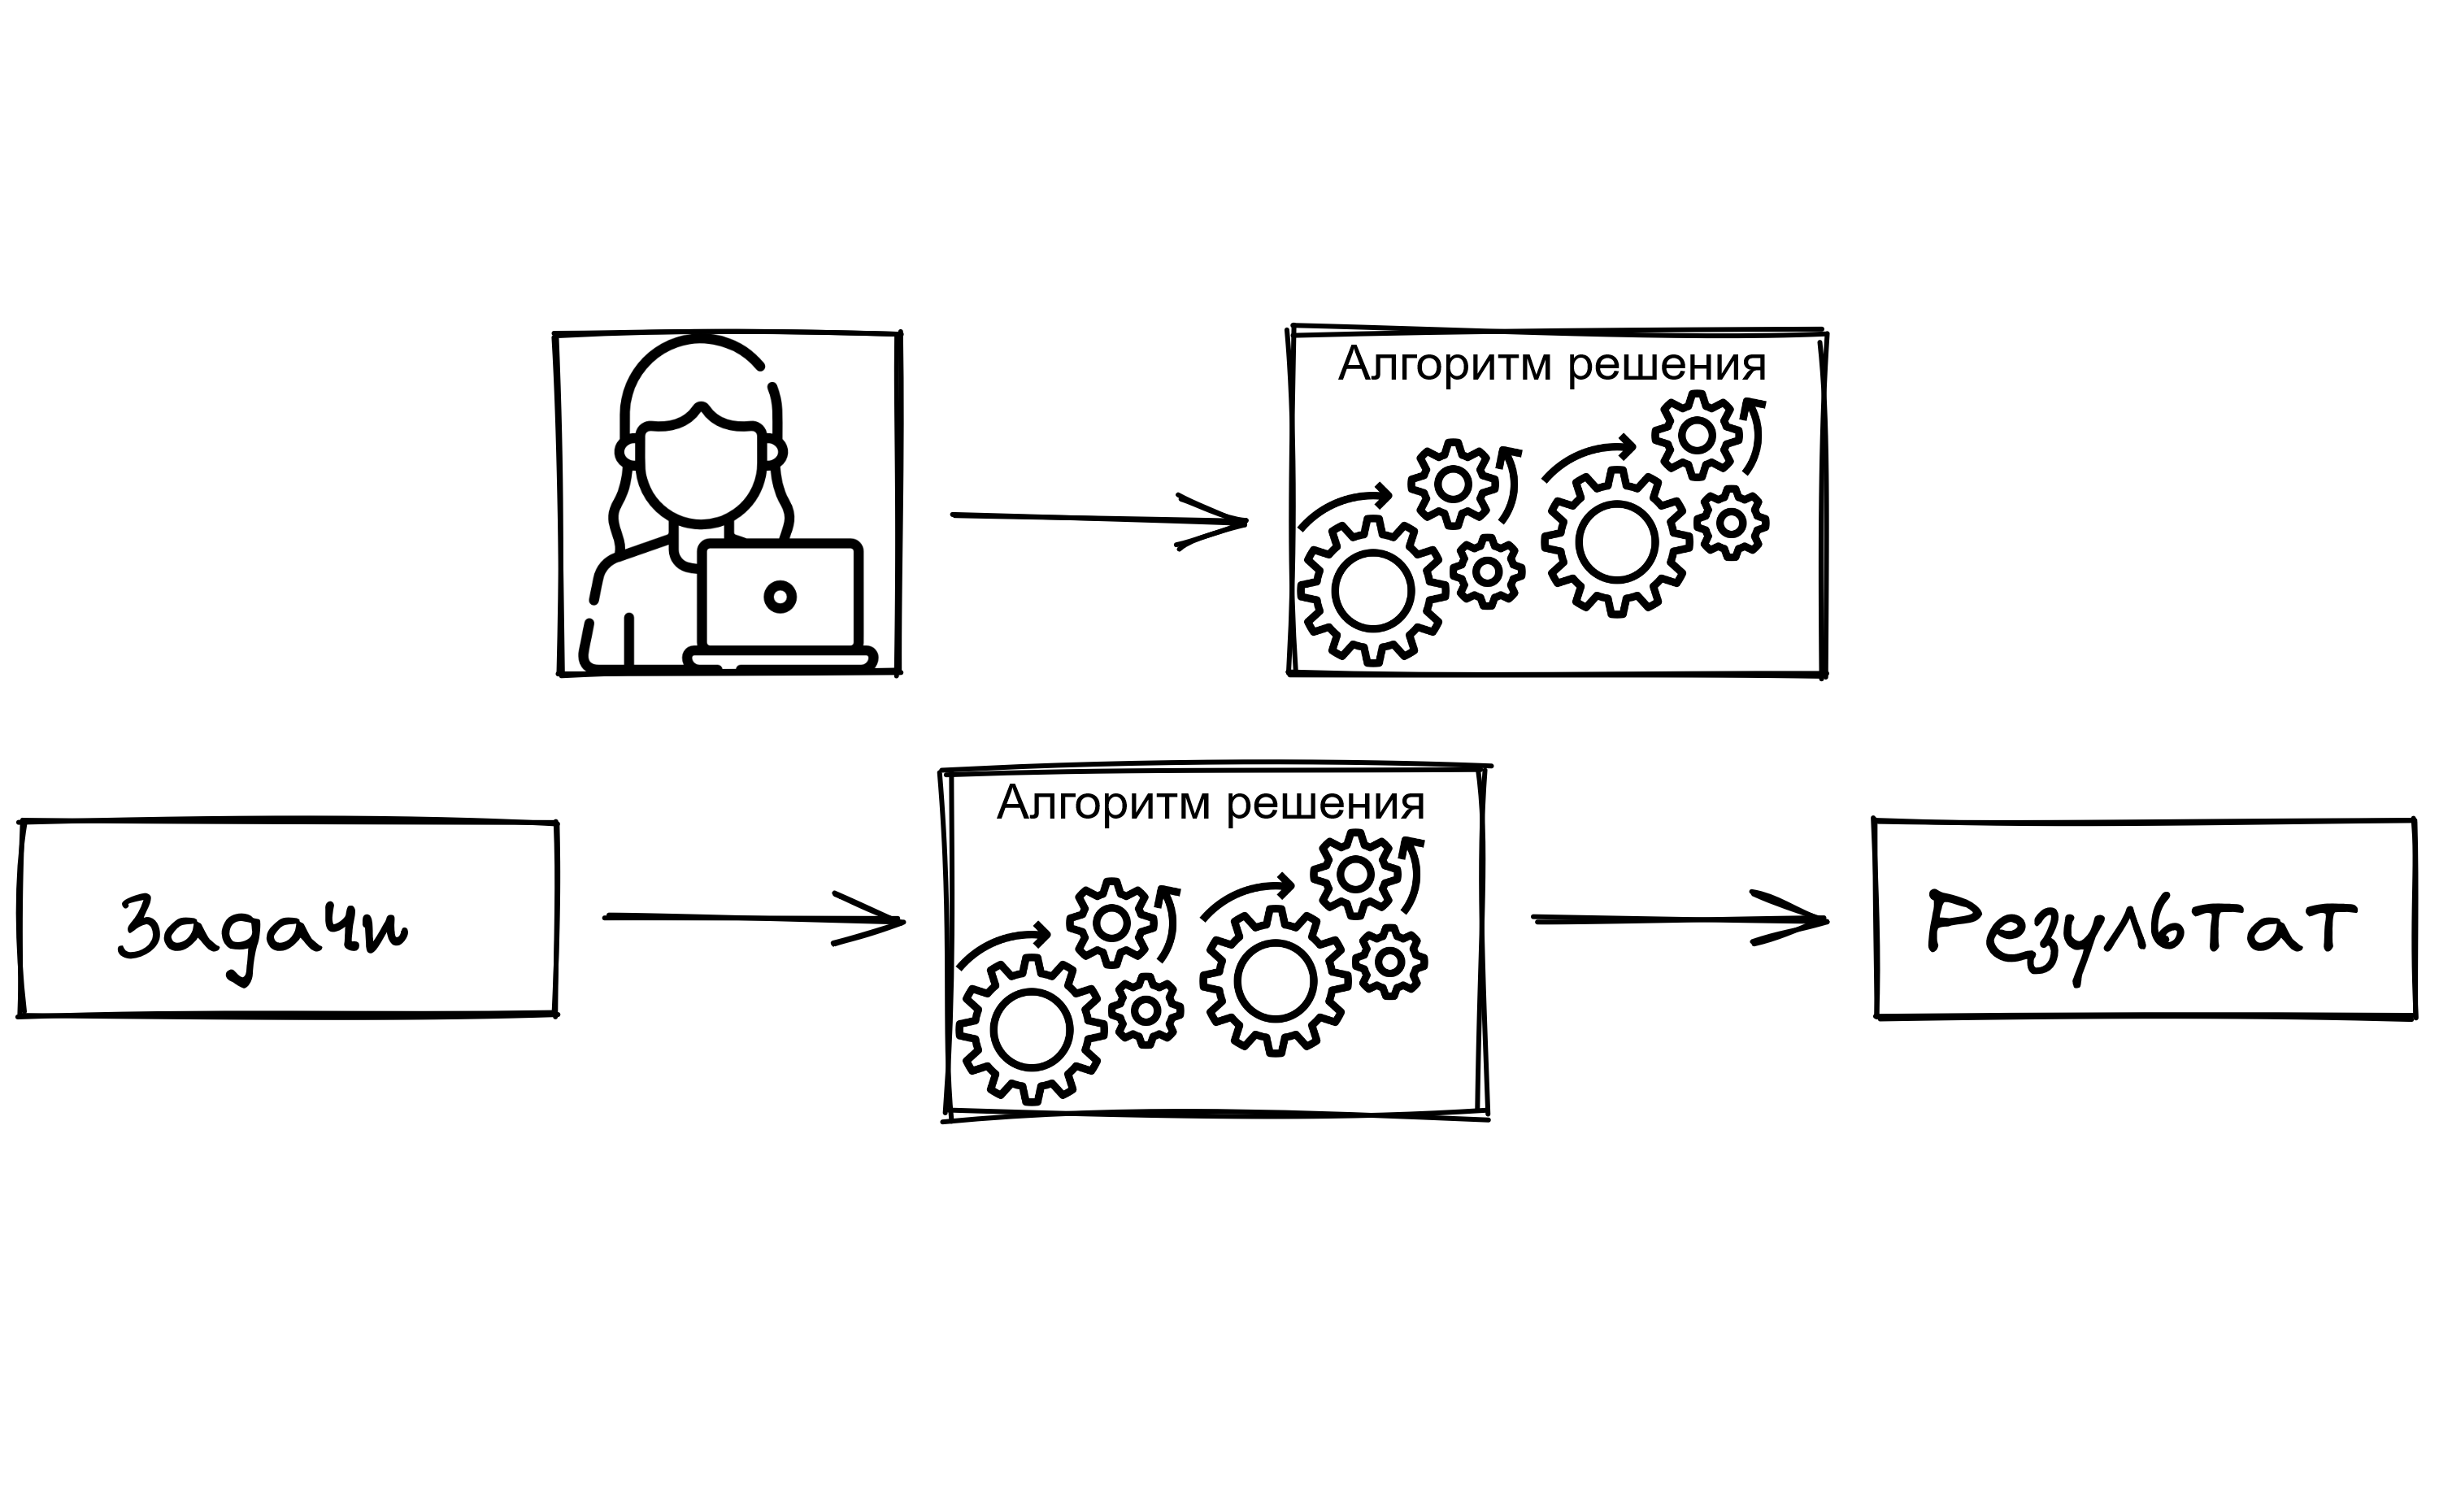
\includegraphics[width=\linewidth]{graphs/fig1_1.jpg}
        \end{column}
        \begin{column}{.49\linewidth}
            \centering
            Machine Learning
            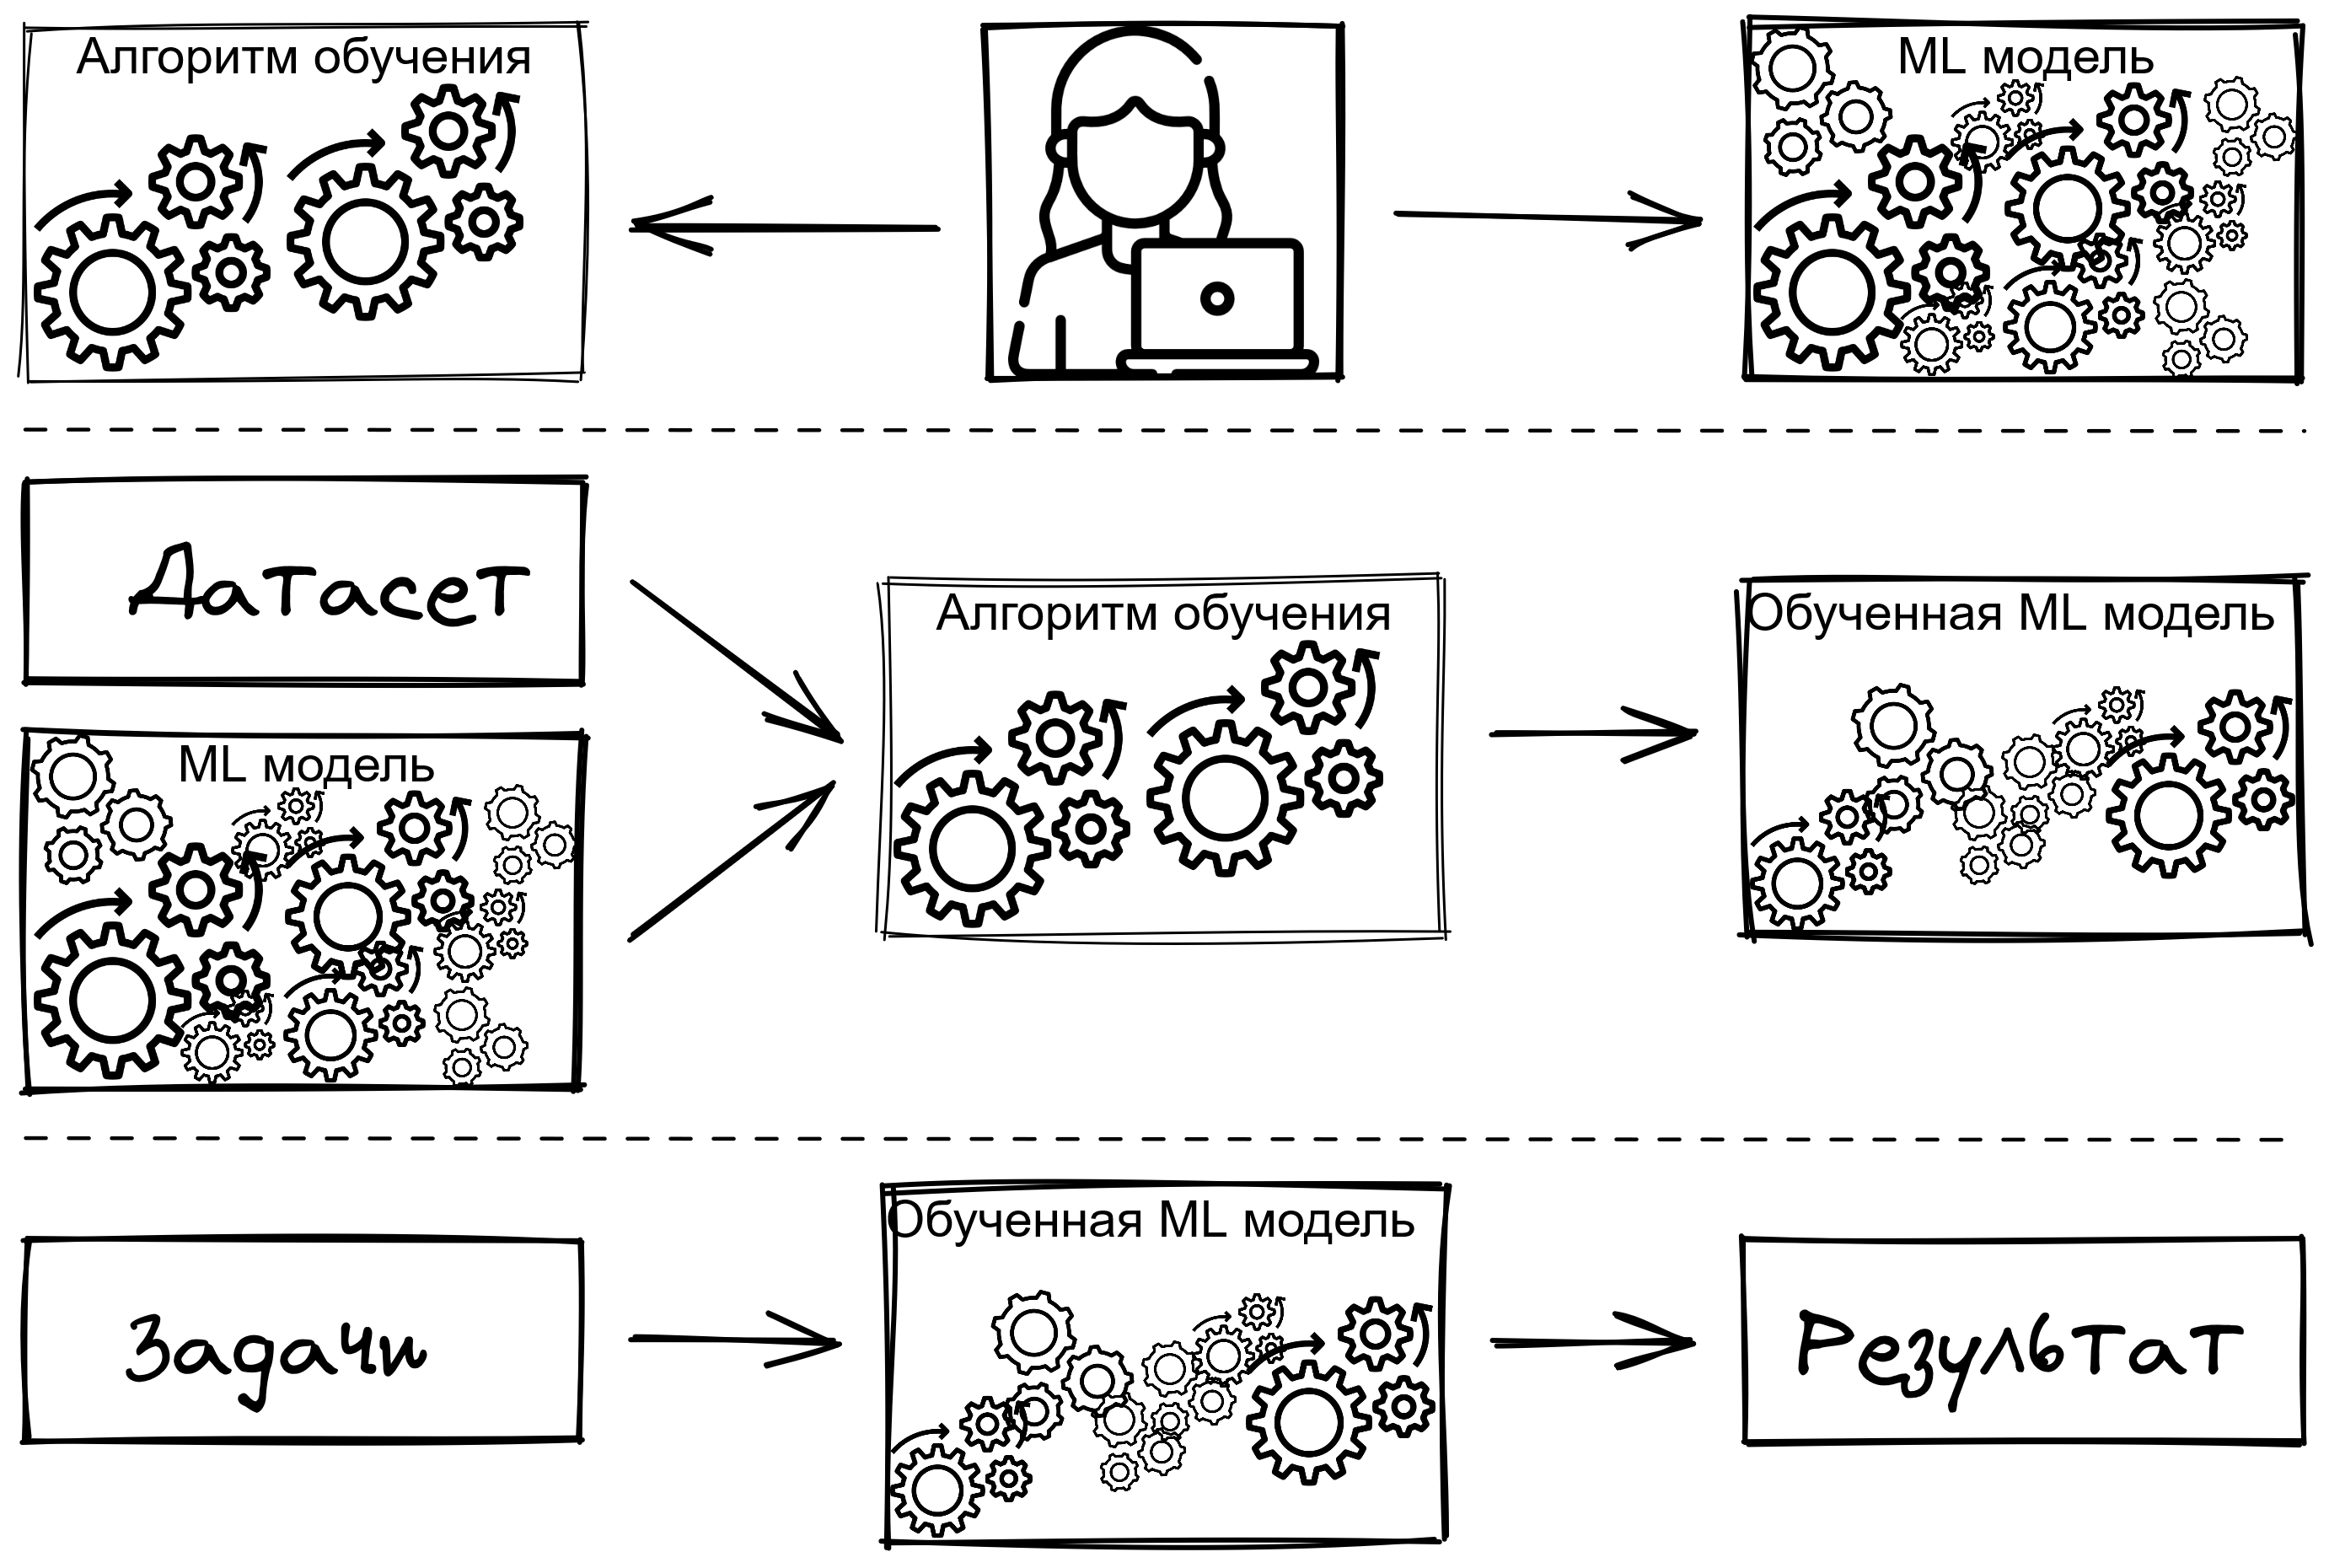
\includegraphics[width=\linewidth]{graphs/fig1_2.jpg}
        \end{column}
    \end{columns}
\end{frame}

\begin{frame}{Когда применим ML?}
    \begin{outline}
        \1 Модели машинного обучения пытаются \textbf{восстанавливать закономерности} на
        основе \textbf{данных}, а не исходя из понимания природы или здравого смысла
        \1 ``Золотое'' правило машинного обучения
    \end{outline}
    \begin{center}
        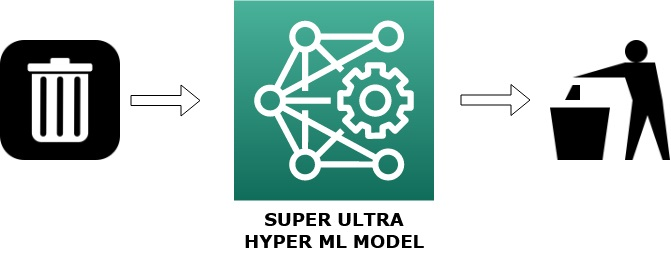
\includegraphics[width=.49\linewidth]{graphs/fig2.jpg} \\
        garbade in --- garbage out
    \end{center}
\end{frame}

\begin{frame}{История}
    \centering
    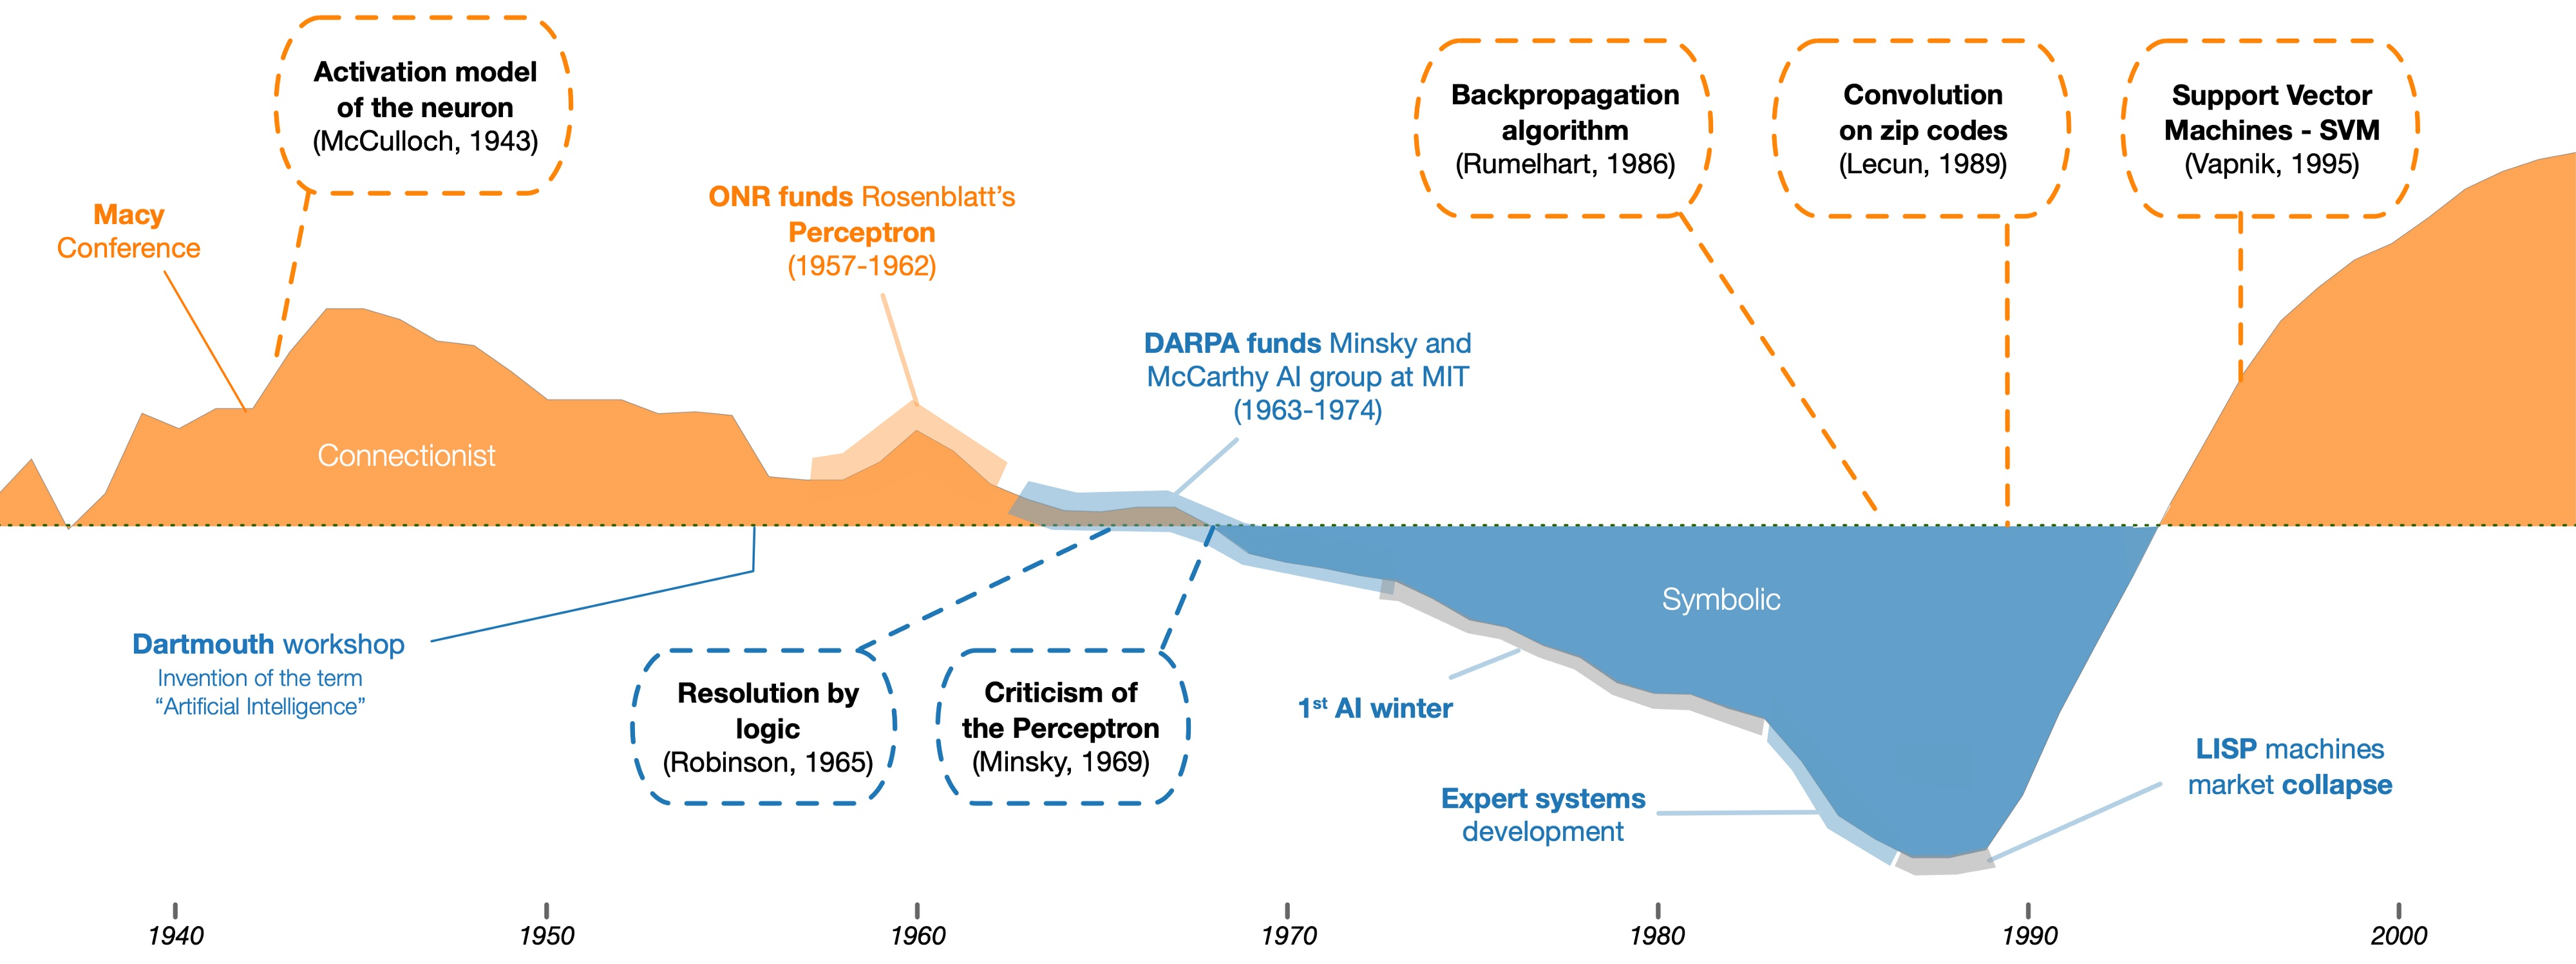
\includegraphics[width=\linewidth]{graphs/fig3.jpg} \\
    82 года истории исследований AI
\end{frame}

\begin{frame}{Задачи машинного обучения}
    \centering
    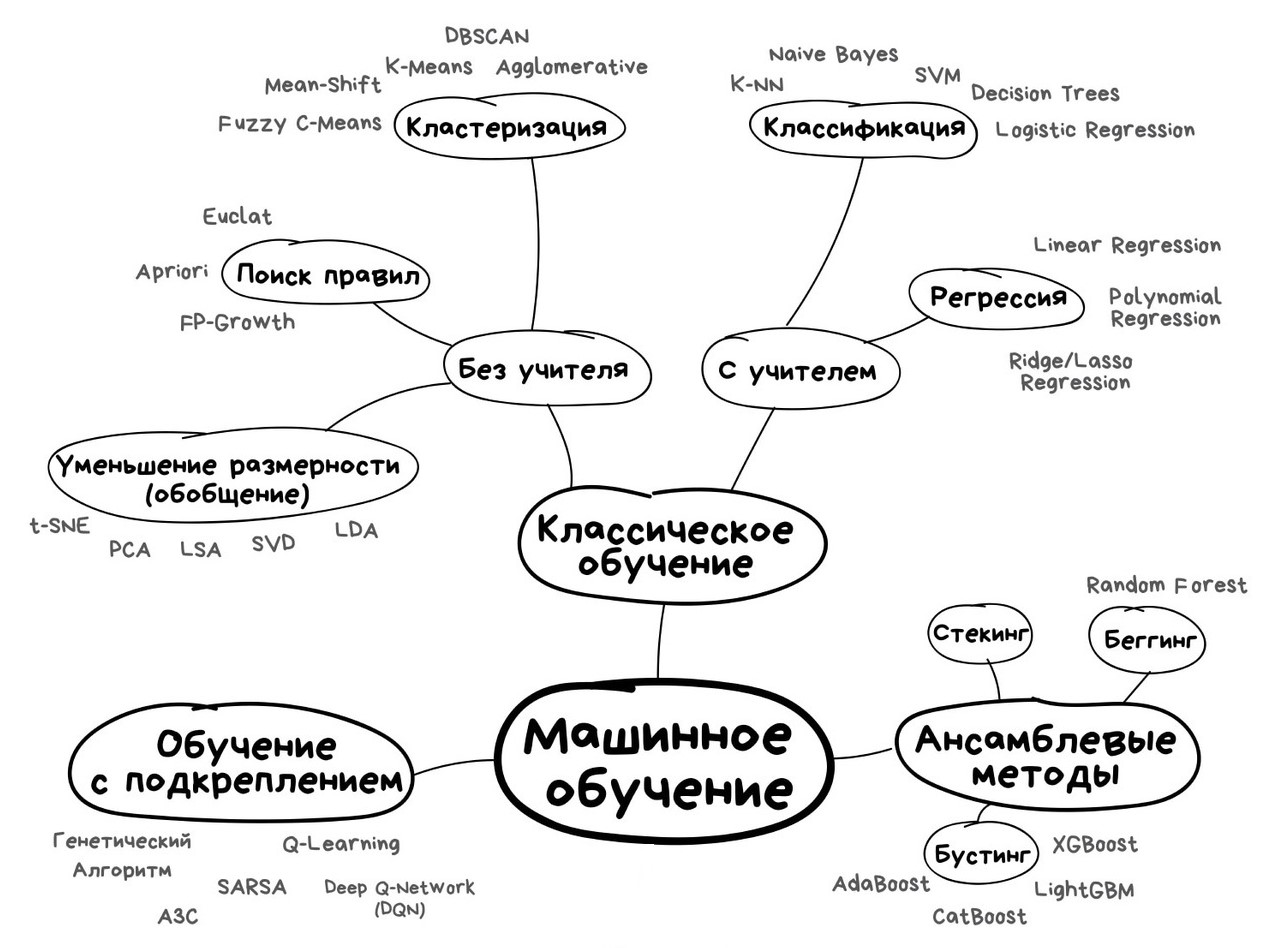
\includegraphics[width=.65\linewidth]{graphs/fig4.jpg}
\end{frame}

\begin{frame}{Задачи машинного обучения}
    \centering
    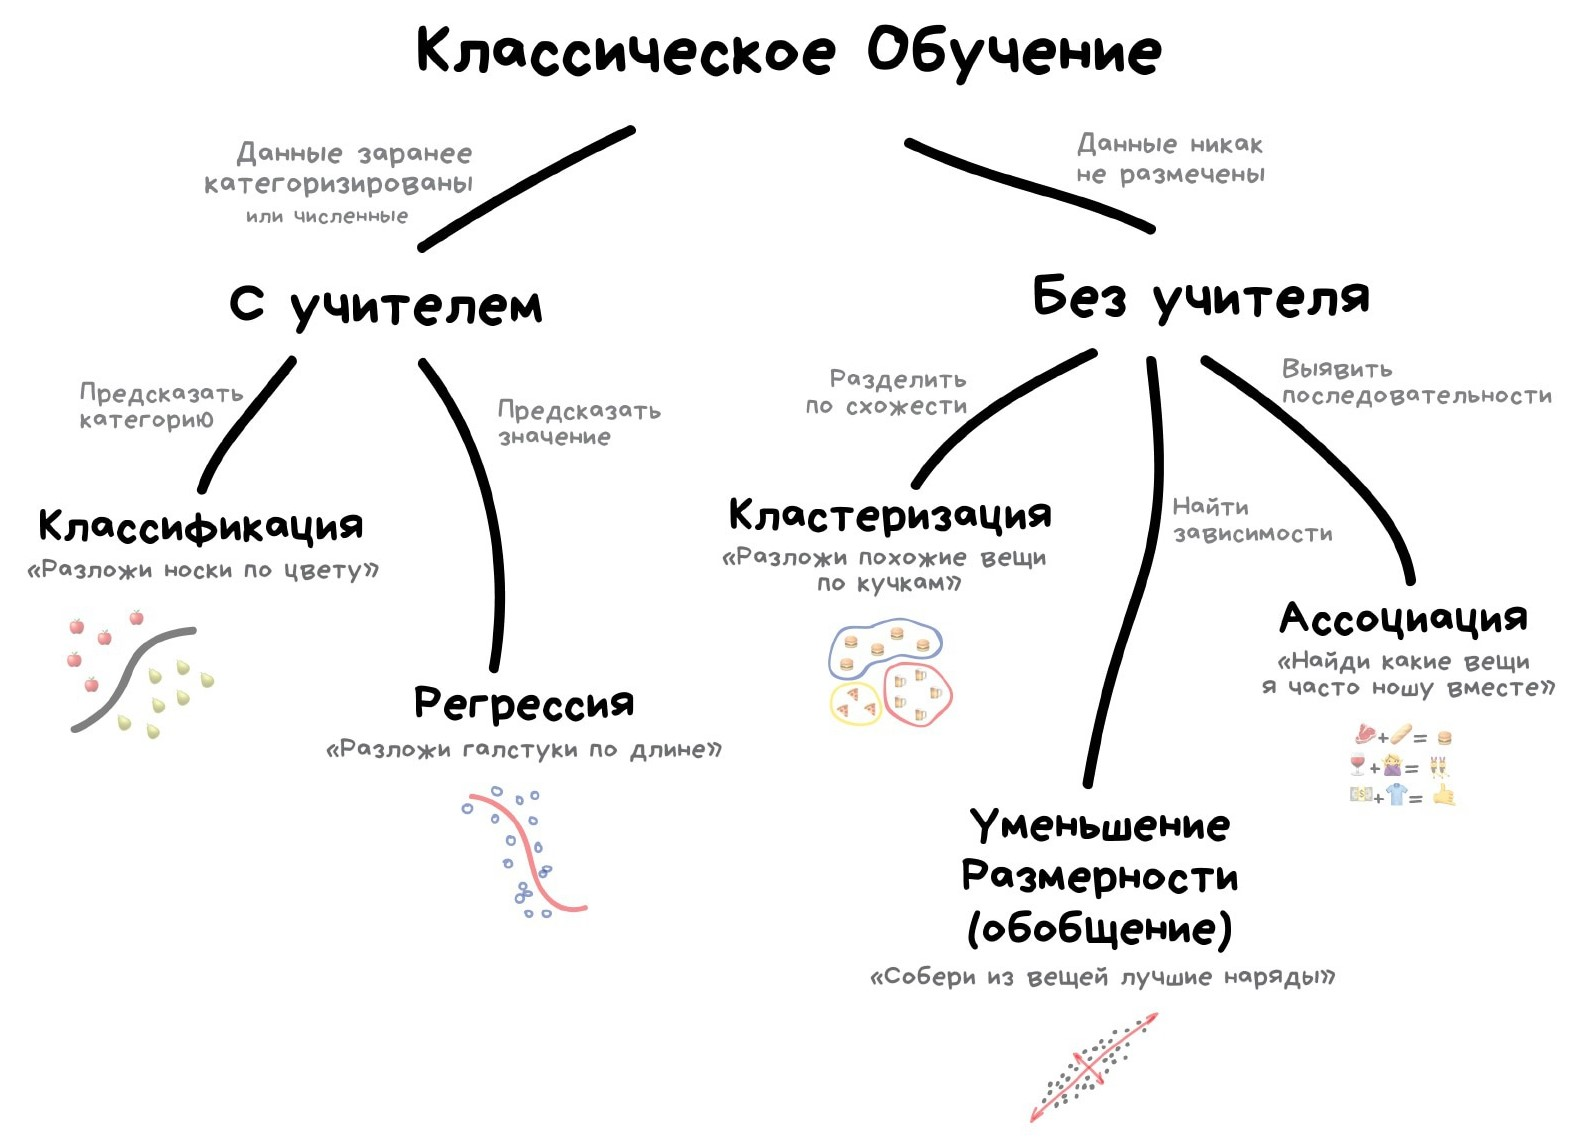
\includegraphics[width=.67\linewidth]{graphs/fig5.jpg}
\end{frame}

\begin{frame}{Классификация и регрессия}
    \centering
    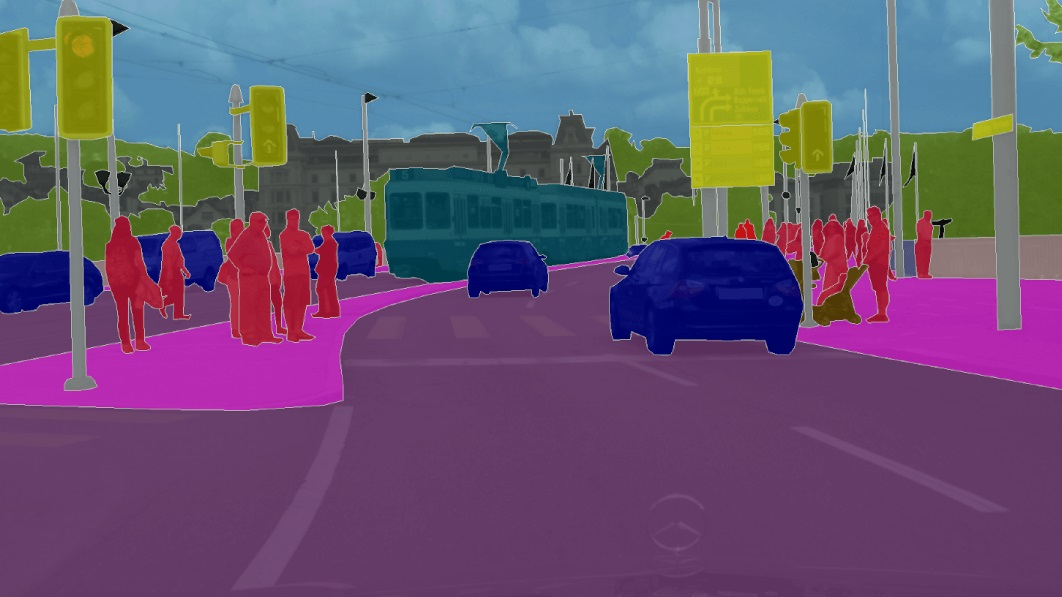
\includegraphics[width=.78\linewidth]{graphs/fig6.jpg} \\
    Задача семантической сегментации (semantic segmentation)
\end{frame}

\begin{frame}{Классификация и регрессия}
    \centering
    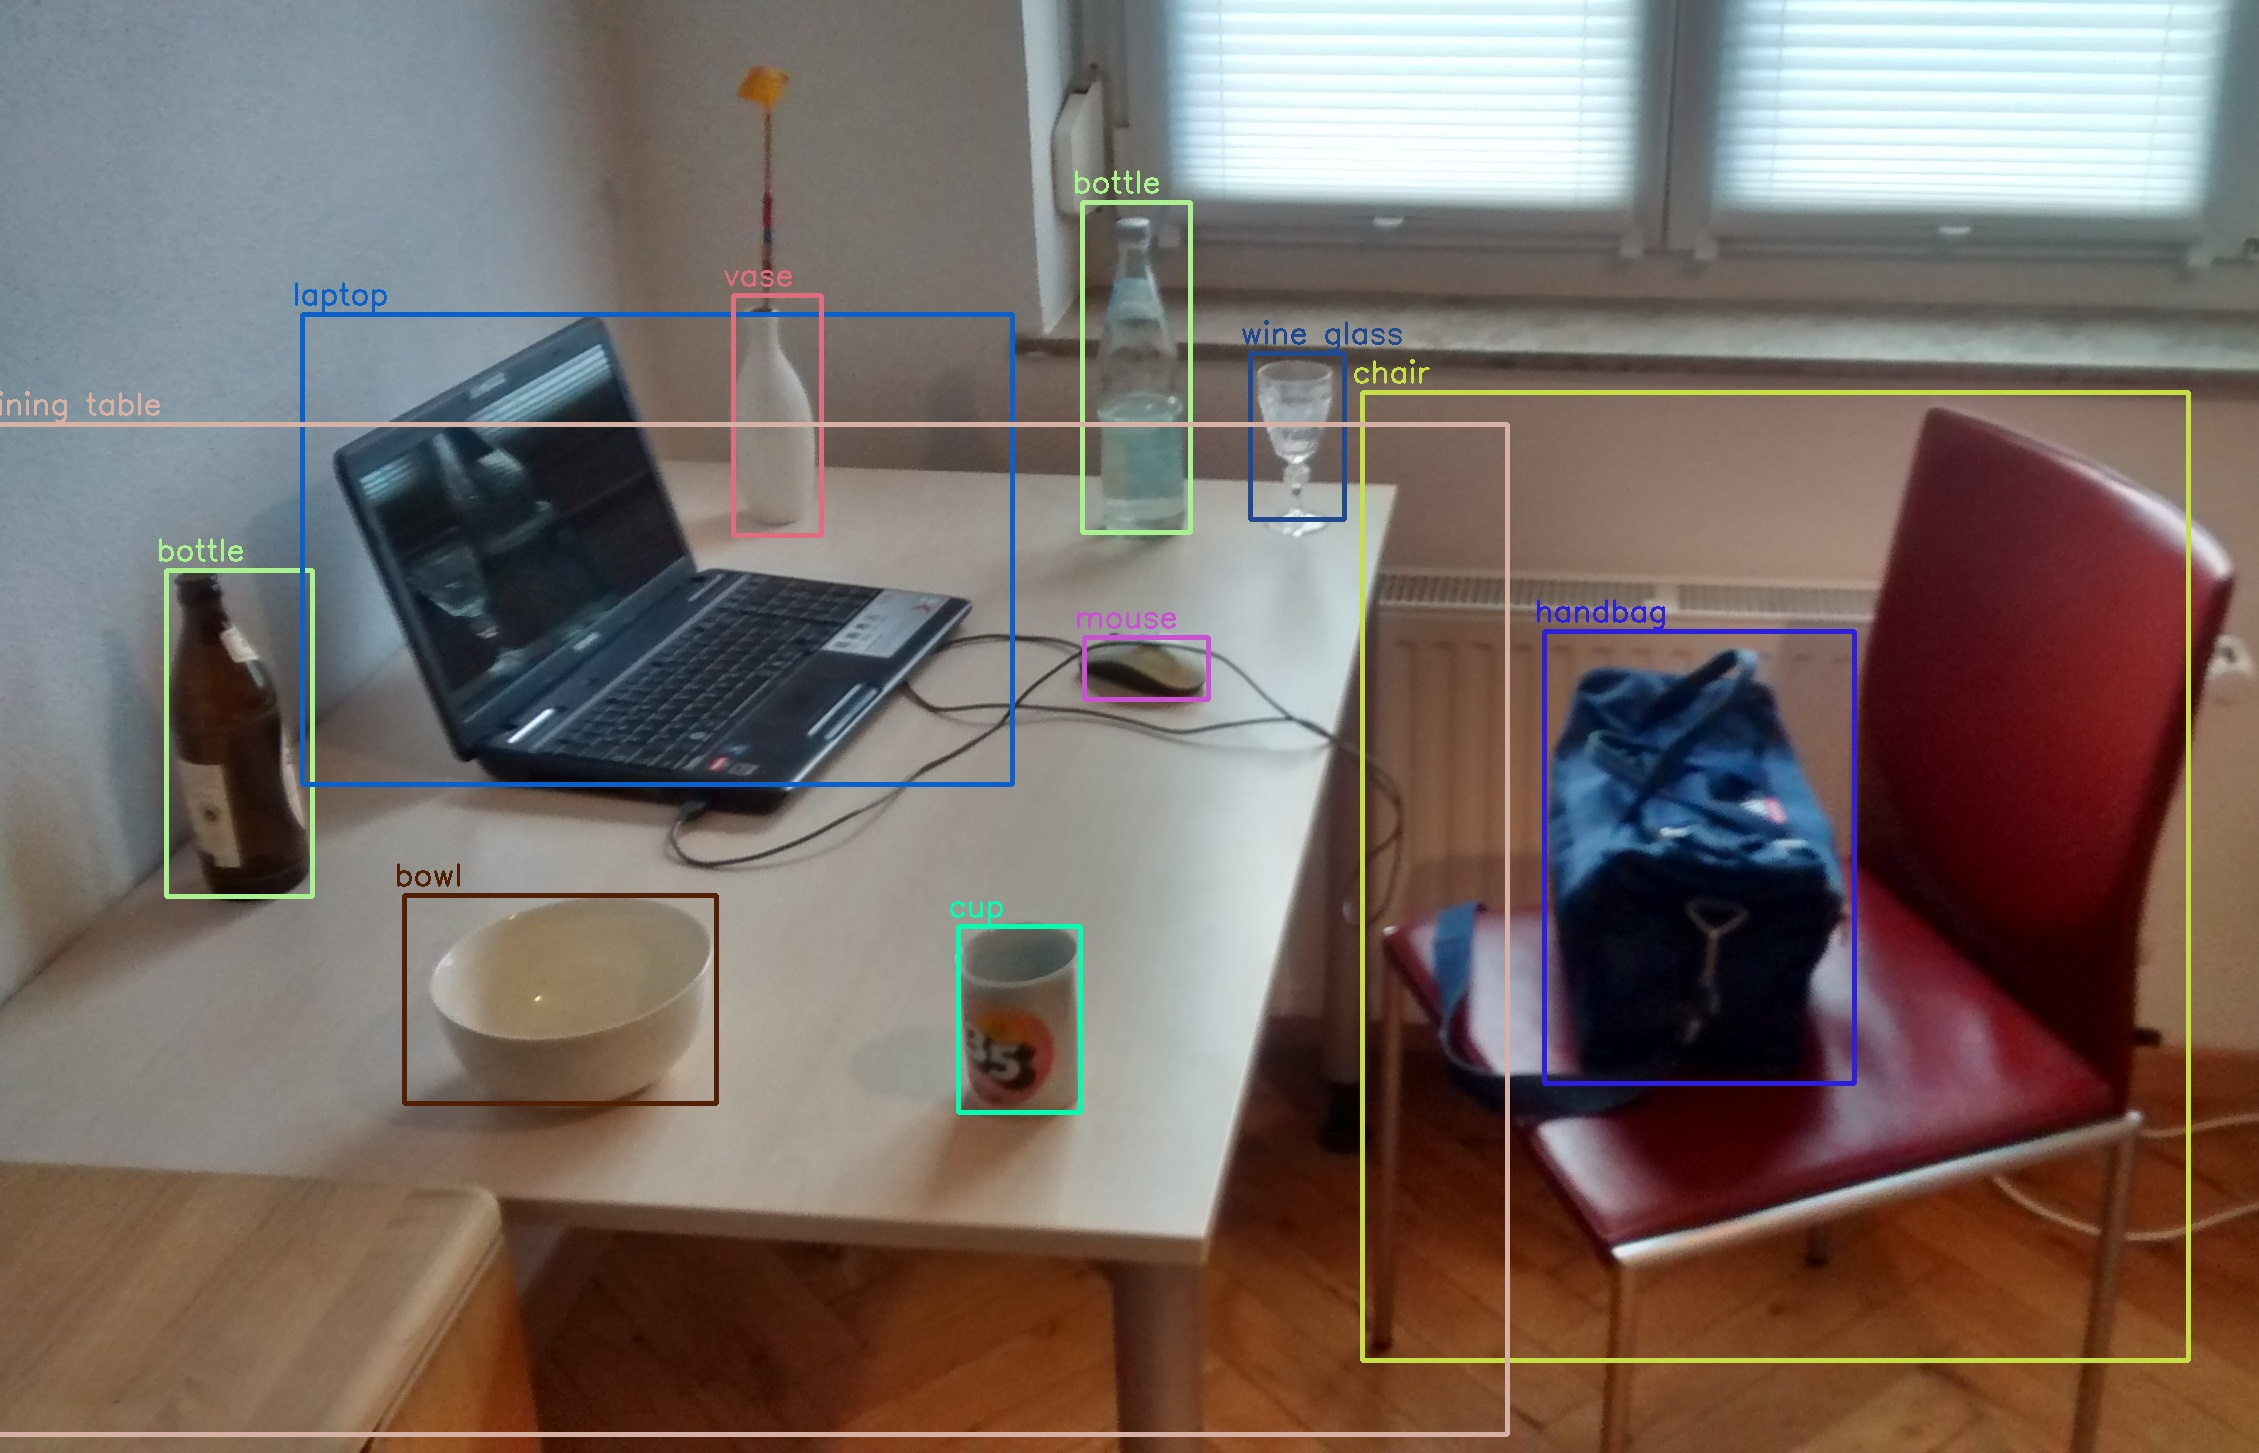
\includegraphics[width=.68\linewidth]{graphs/fig7.jpg} \\
    Задача детектирования объектов (object detection)
\end{frame}

\begin{frame}{План СПК}
    \begin{columns}
        \begin{column}{.5\linewidth}
            {\tiny
                \begin{outline}
                    \1 \textit{10.09 Вводная лекция}
                    \1 \textbf{17.09 Вводная лекция pt.2 / Работа с данными в Python. Семинар}
                    \1 24.09 Работа с данными в Python. Семинар pt.2
                    \1 01.10 Линейная регрессия. Лекция
                    \1 08.10 Линейная регрессия. Семинар
                    \1 15.10 Хакатон
                    \1 22.10 Линейная классификация. Лекция
                    \1 29.10 Линейная классификация. Семинар
                    \1 Задание на каникулы
                    \1 12.11 Искуственные нейронные сети. Лекция
                    \1 19.11 Полносвязные нейронные сети. Семинар
                    \1 26.11 Основы фреймворка PyTorch. Семинар
                    \1 03.12 Сверточные нейронные сети. Лекция
                    \1 10.12 Архитектуры CNN, transfer learning. Лекция / семинар
                    \1 17.12 Методы улучшения качества сетей. Лекция
                    \1 24.12 Финальное задание
                \end{outline}
            }
        \end{column}
        \begin{column}{.49\linewidth}
            
\includegraphics[width=.55\linewidth]{graphs/fig8_1.jpg}
            
\includegraphics[width=.55\linewidth]{graphs/fig8_2.jpg}
            
\includegraphics[width=.55\linewidth]{graphs/fig8_3.jpg}
            
\includegraphics[width=.55\linewidth]{graphs/fig8_4.jpg}
        \end{column}
    \end{columns}
\end{frame}

\begin{frame}{Ссылка на семинар}
    \centering
    \LARGE https://bit.ly/3BrjTaP
\end{frame}

\end{document}